\section{Programação Visual e Ambientes Baseados em Fluxos}

\subsection{Conceitos de programação visual}

A programação visual é uma abordagem de desenvolvimento na qual a lógica computacional é representada por elementos gráficos, como blocos, nós e conexões, em vez de ser expressa exclusivamente por código textual. Essa forma de representação busca tornar a construção e compreensão de sistemas mais intuitiva, permitindo que processos e comportamentos sejam visualizados de maneira direta.

Conforme \citeonline{myers1990}, ambientes de programação visual foram desenvolvidos para facilitar a interação com sistemas computacionais por meio de representações gráficas da lógica. Embora utilizem elementos visuais, esses ambientes continuam baseados nos mesmos princípios computacionais encontrados nas linguagens tradicionais de programação.

Essa característica revela um aspecto central da programação visual: por se apoiar nos mesmos princípios computacionais das linguagens textuais, ela demonstra que um mesmo comportamento pode ser implementado tanto por código quanto por fluxos visuais. Essa equivalência é o que torna os ambientes visuais especialmente relevantes para esta pesquisa, e as próximas subseções examinam suas principais manifestações --- os fluxogramas, os blueprints e as plataformas de baixo código.

\subsection{Fluxogramas e representação de algoritmos}

Os fluxogramas constituem uma das formas mais tradicionais de representação visual de algoritmos. Por meio de símbolos padronizados e conexões direcionais, eles permitem representar decisões, processos e fluxos de execução de maneira gráfica, facilitando a compreensão da lógica computacional.

Além de sua função representativa, os fluxogramas são amplamente utilizados para documentar e comunicar algoritmos durante o desenvolvimento de software. Sua estrutura visual torna mais acessível a compreensão do comportamento de sistemas computacionais, especialmente em etapas de análise, planejamento e documentação.

Cabe destacar, no entanto, que os fluxogramas possuem caráter essencialmente descritivo. Eles representam a lógica de um algoritmo para fins de compreensão e comunicação, mas não constituem, por si sós, um mecanismo de execução: a lógica representada precisa ser posteriormente traduzida em código para ser executada por um sistema computacional. Essa distinção entre representar e executar é relevante para esta pesquisa, pois diferencia os fluxogramas de outras representações visuais, como os blueprints, capazes de executar diretamente a lógica que descrevem, conforme discutido na seção seguinte.


A Figura \ref{fig:logica_central_codigo_fluxograma} apresenta a lógica computacional como elemento central entre diferentes formas de representação. Nesse contexto, tanto o código-fonte quanto os fluxogramas podem expressar uma mesma estrutura lógica, diferenciando-se apenas pela forma como essa informação é apresentada ao desenvolvedor.

\begin{figure}[H]
    \centering
    \caption{Relação entre diferentes formas de representação da lógica computacional.}
    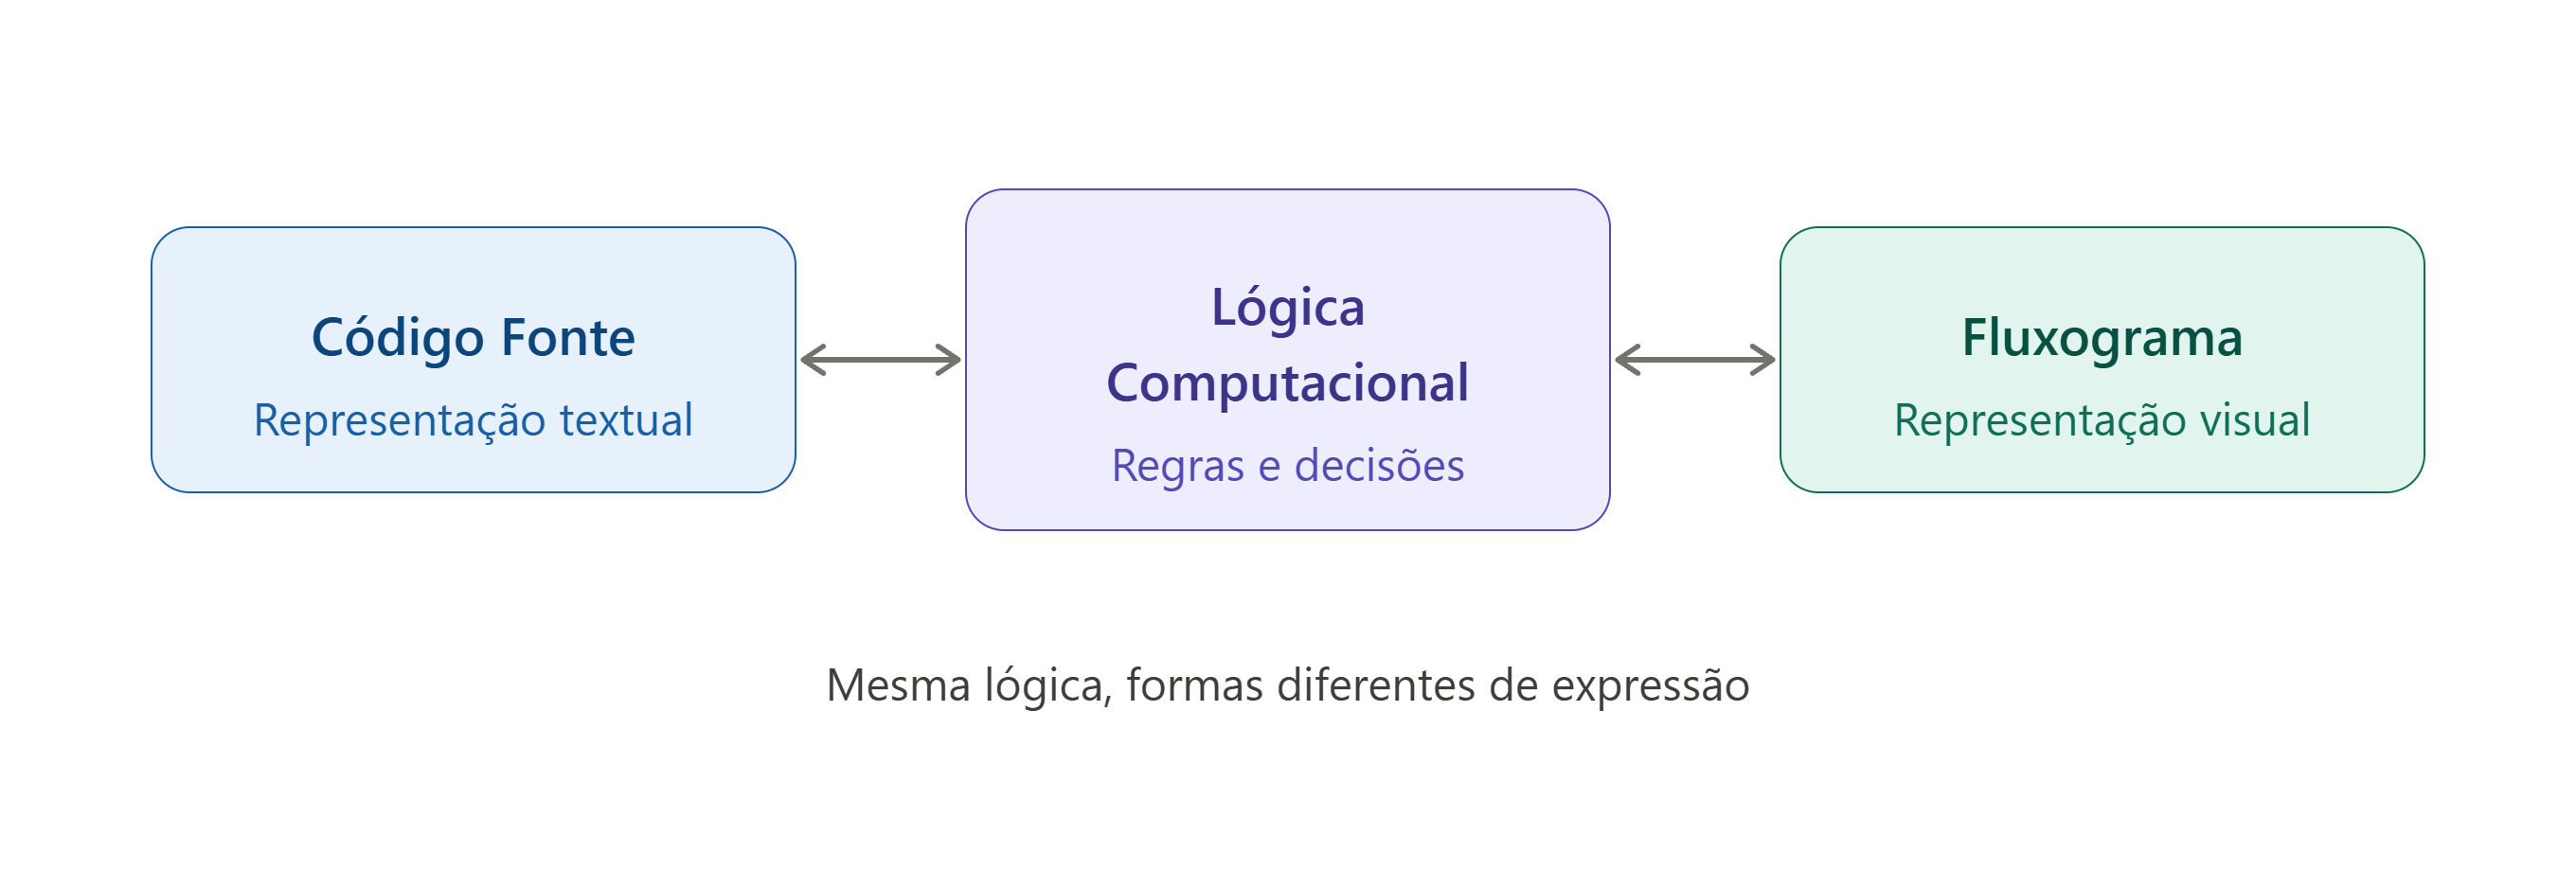
\includegraphics[width=0.85\textwidth]{images/logica_central_codigo_fluxograma.png}
    \legend{Fonte: elaboração do autor com base em \citeonline{abelson1996} e \citeonline{knuth1968}.}
    \label{fig:logica_central_codigo_fluxograma}
\end{figure}

\subsection{Blueprints e sistemas baseados em nós}

Os \textit{blueprints} e sistemas baseados em nós representam uma evolução dos modelos tradicionais de programação visual \cite{romero2014blueprint}. Nesses ambientes, a lógica computacional é construída por meio da conexão entre elementos gráficos denominados nós, que representam operações, eventos, decisões ou fluxos de dados.

Diferentemente dos fluxogramas, que possuem principalmente função descritiva e documental, os sistemas baseados em nós permitem a execução direta da lógica construída visualmente. Dessa forma, o fluxo visual deixa de ser apenas uma representação e passa a atuar como mecanismo efetivo de desenvolvimento de software.

Um dos exemplos mais conhecidos dessa abordagem é o sistema Blueprint da Unreal Engine, utilizado para o desenvolvimento de jogos e aplicações interativas. Nesse ambiente, programadores e designers podem construir comportamentos complexos por meio da conexão visual de nós, reduzindo a necessidade de escrita manual de código textual.

Essa característica reforça a hipótese de que a lógica computacional pode ser separada de sua forma de representação. Embora os \textit{blueprints} utilizem elementos visuais, os comportamentos implementados seguem os mesmos princípios algorítmicos encontrados nas linguagens de programação tradicionais.

A documentação oficial da Epic Games \cite{epic_blueprint} descreve o sistema Blueprint como uma interface de scripting visual que disponibiliza recursos de programação por meio de nós conectados. A solidez lógica dessa abordagem é evidenciada por trabalhos que demonstram ser possível aplicar verificação formal sobre scripts construídos em blueprints. \citeonline{wayama2022blueprint}, por exemplo, aplicaram model checking a programas desenvolvidos no Blueprint da Unreal Engine 5, evidenciando que a lógica representada visualmente pode ser formalmente analisada. Isso reforça a ideia central desta pesquisa: a de que a representação visual expressa uma estrutura lógica computacional bem definida, e não apenas um recurso gráfico de apoio.

Nesse contexto, os sistemas baseados em nós demonstram que diferentes formas de representação podem expressar uma mesma estrutura lógica, aspecto que se relaciona diretamente com a proposta desta pesquisa. A Figura \ref{fig:blueprint_if_idade} ilustra esse conceito por meio do mesmo exemplo lógico apresentado na Figura \ref{fig:figura1_traducao_representacoes} --- a condição \texttt{if idade >= 18} ---, desta vez expressa no formato de nós conectados característico dos sistemas blueprint. Embora a representação seja visualmente distinta do código textual e do fluxograma, o comportamento lógico subjacente permanece idêntico.

\begin{figure}[H]
    \centering
    \caption{Exemplo de lógica computacional representada por meio de um sistema visual baseado em nós (blueprint).}
    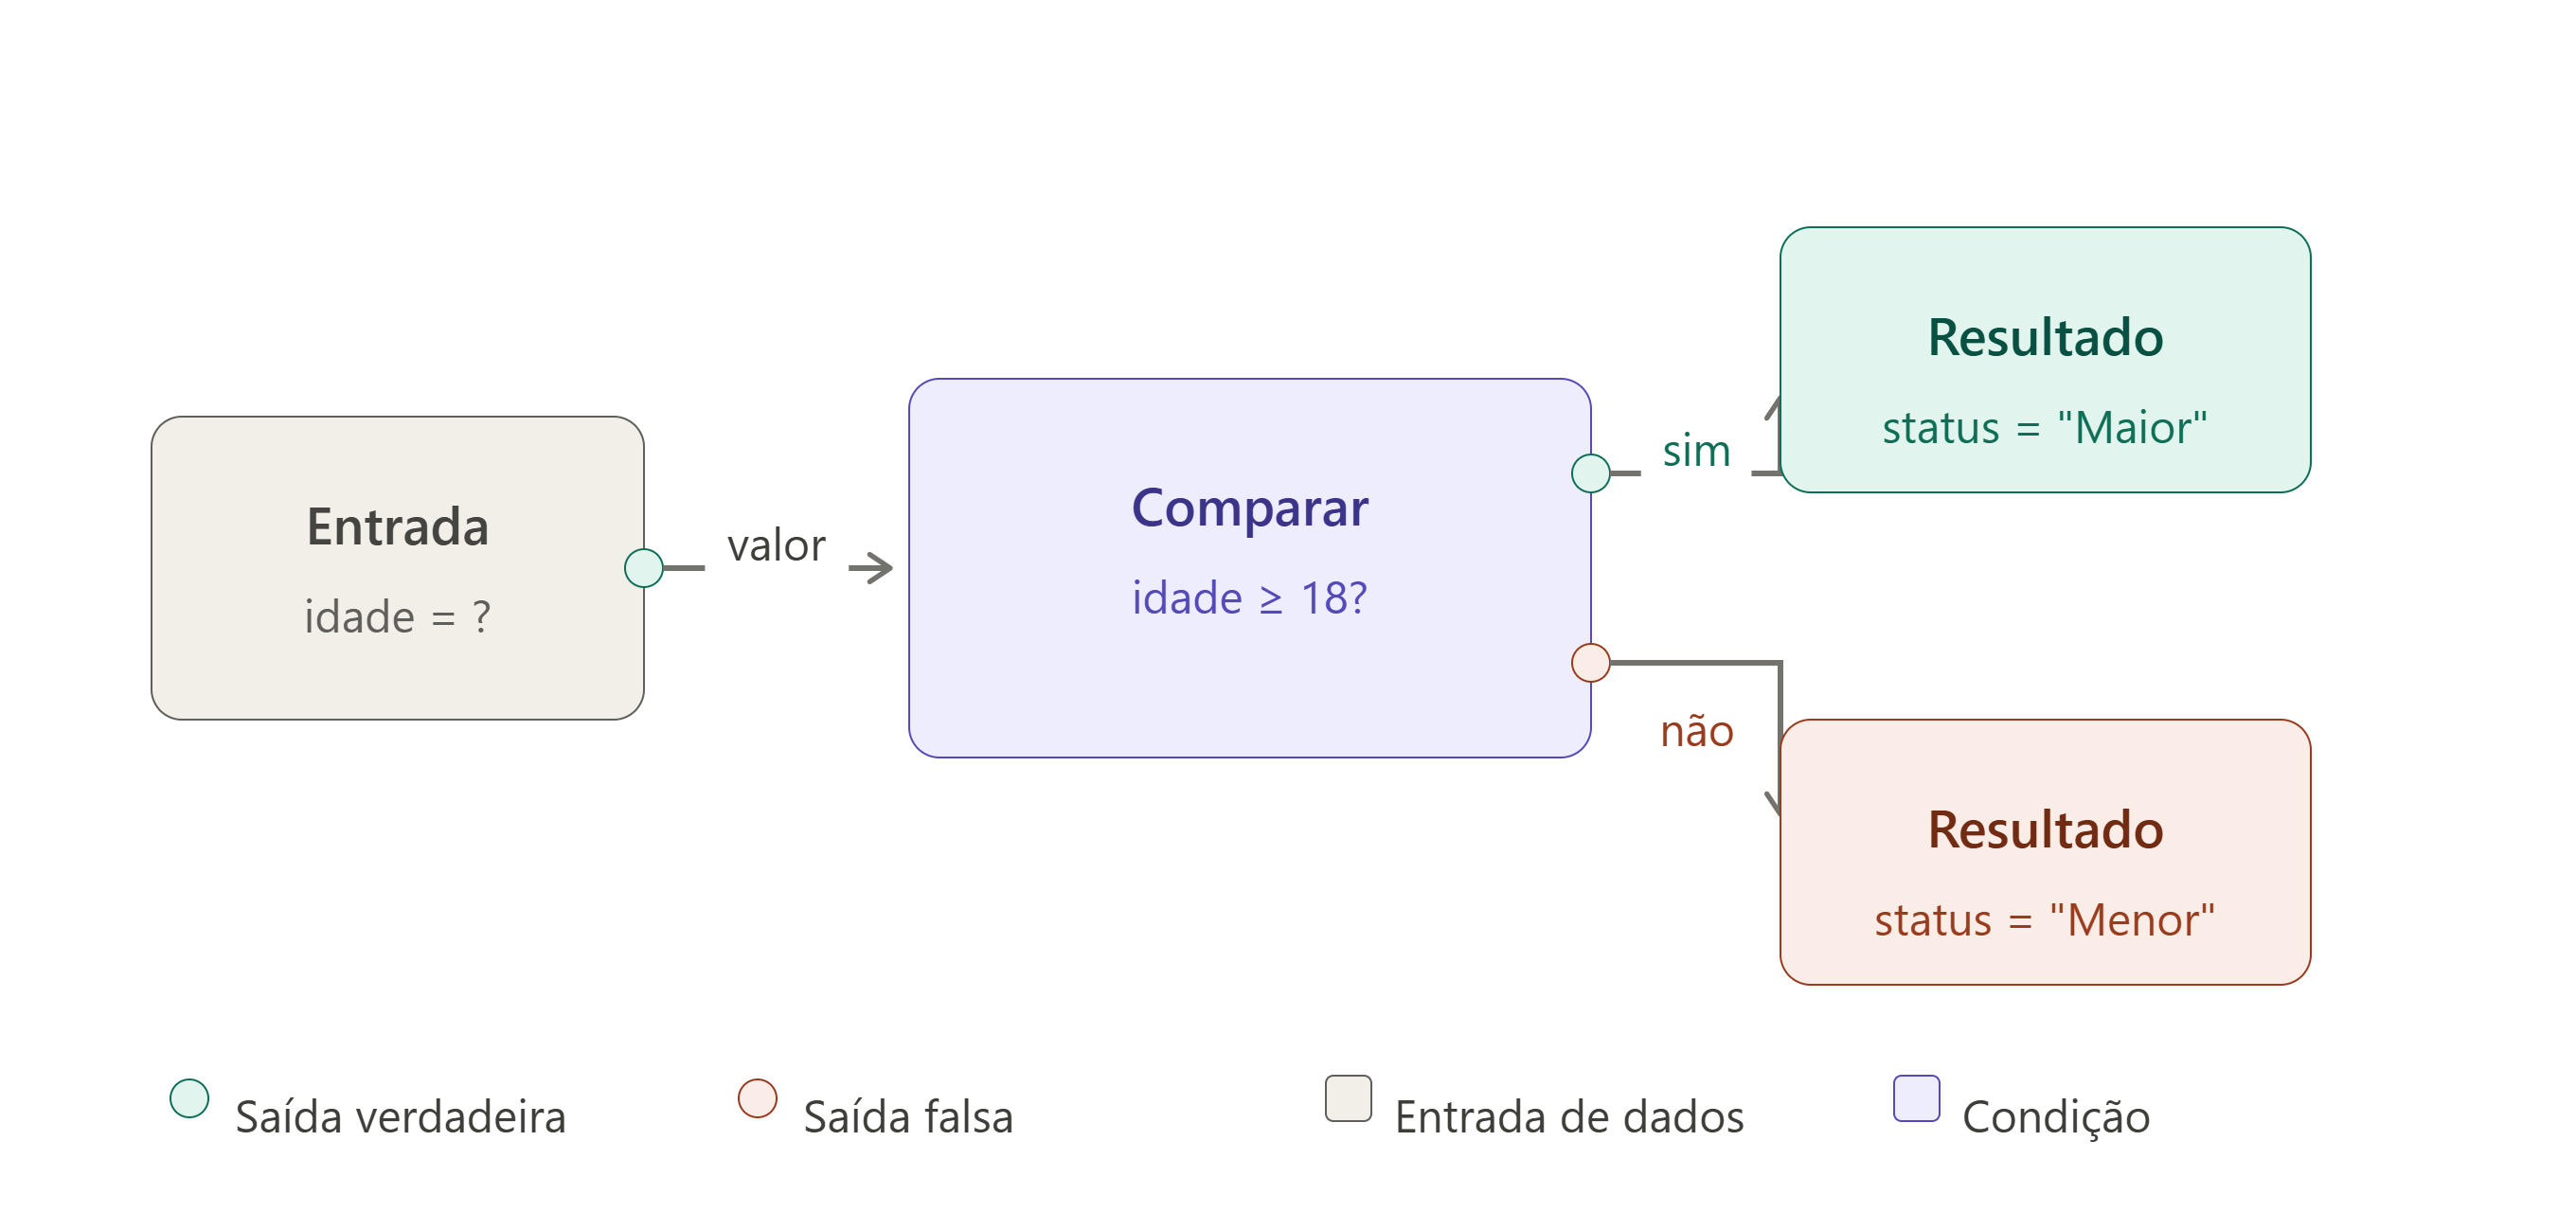
\includegraphics[width=\textwidth]{images/blueprint_if_idade.png}
    \legend{Fonte: elaboração do autor com base em \citeonline{romero2014blueprint} e \citeonline{epic_blueprint}.}
    \label{fig:blueprint_if_idade}
\end{figure}

\subsection{Plataformas Low-Code e No-Code}

As plataformas \textit{Low-Code} e \textit{No-Code} surgiram como uma evolução dos ambientes de programação visual, buscando reduzir a complexidade do desenvolvimento de software por meio de interfaces gráficas e componentes reutilizáveis. Nessas plataformas, grande parte da lógica é construída por meio da conexão entre blocos, fluxos e elementos visuais, diminuindo a necessidade de escrita manual de código.

A utilização de representações visuais para construção de sistemas computacionais contribui para ampliar a acessibilidade ao desenvolvimento de software, permitindo que usuários com diferentes níveis de conhecimento técnico participem da criação de soluções digitais \cite{myers1990}.

Nesse contexto, plataformas como \textit{n8n}, \textit{Node-RED}, \textit{Microsoft Power Automate} e outras ferramentas de automação utilizam fluxos visuais para representar processos, integrações e comportamentos computacionais. Embora apresentem interfaces simplificadas, essas plataformas continuam baseadas nos mesmos princípios lógicos encontrados nas linguagens tradicionais de programação \cite{silva2023lowcode}.

Cada uma dessas ferramentas adota uma forma própria de representar a lógica, ainda que compartilhem o princípio comum dos fluxos visuais. No \textit{n8n}, a lógica é organizada em nós que atuam como blocos de construção de um fluxo de trabalho, responsáveis por iniciar a execução, buscar e enviar dados e manipular informações \cite{n8ndocs}. O \textit{Node-RED}, por sua vez, baseia-se na programação orientada a eventos e no encadeamento de nós, sendo amplamente aplicado à integração de dispositivos e à Internet das Coisas \cite{nodereddocs}. Já o \textit{Microsoft Power Automate} estrutura a lógica em fluxos compostos por gatilhos, que iniciam a execução a partir de um evento, e ações, que definem as operações realizadas em seguida \cite{powerautomatedocs}. Apesar das diferenças visuais e estruturais entre essas representações, todas expressam decisões, condições e sequências de execução, evidenciando que uma mesma lógica computacional pode assumir formas distintas conforme o ambiente utilizado.


\subsubsection*{Síntese da seção}

A análise dos ambientes apresentados demonstra que a lógica computacional pode ser representada por diferentes modelos visuais (fluxogramas, blueprints e plataformas \textit{Low-Code} ou \textit{No-Code}) sem perder sua capacidade de expressar algoritmos, decisões e fluxos de execução. Embora cada abordagem possua características e objetivos distintos, todas compartilham um princípio comum: a utilização de elementos visuais para representar estruturas lógicas, sem alteração de seu significado fundamental.

Essa constatação fornece suporte teórico à hipótese investigada nesta pesquisa e estabelece a base para o capítulo seguinte, no qual se discute como essa estrutura lógica comum pode atuar como elemento intermediário na tradução entre diferentes representações computacionais.